\begin{center}
      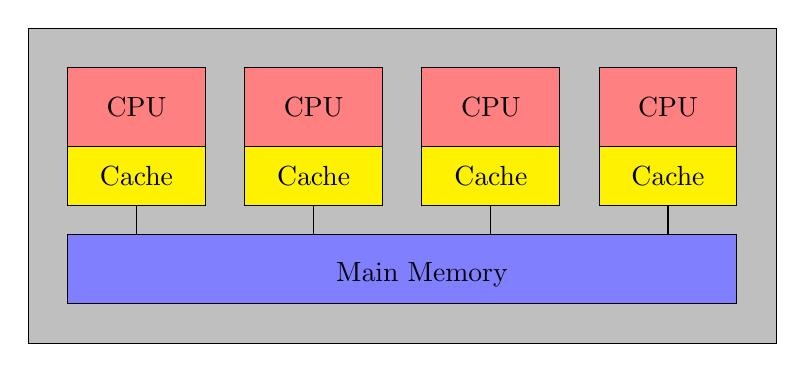
\begin{tikzpicture}[scale=0.5]
        \filldraw[fill=gray!50!white] (0,0) rectangle (19,8);
        \filldraw[fill=blue!50!white] (1,1) rectangle (18,2.75);
        \draw (10,1.75) node {Main Memory};
        % First Core
        \filldraw[fill=yellow] (1,3.5) rectangle (4.5,5.0);
        \draw (2.75,4.25) node {Cache};
        \filldraw[fill=red!50!white] (1,5.0) rectangle (4.5,7.0);
        \draw (2.75,6.0) node {CPU};
        \draw (2.75,3.5) -- (2.75,2.75);
        % Second Core
        \filldraw[fill=yellow] (5.5,3.5) rectangle (9.0,5.0);
        \draw (7.25,4.25) node {Cache};
        \filldraw[fill=red!50!white] (5.5,5.0) rectangle (9.0,7.0);
        \draw (7.25,6.0) node {CPU};
        \draw (7.25,3.5) -- (7.25,2.75);
        % Third Core
        \filldraw[fill=yellow] (10.0,3.5) rectangle (13.5,5.0);
        \draw (11.75,4.25) node {Cache};
        \filldraw[fill=red!50!white] (10.0,5.0) rectangle (13.5,7.0);
        \draw (11.75,6.0) node {CPU};
        \draw (11.75,3.5) -- (11.75,2.75);
        % Fourth Core
        \filldraw[fill=yellow] (14.5,3.5) rectangle (18.0,5.0);
        \draw (16.25,4.25) node {Cache};
        \filldraw[fill=red!50!white] (14.5,5.0) rectangle (18.0,7.0);
        \draw (16.25,6.0) node {CPU};
        \draw (16.25,3.5) -- (16.25,2.75);
      \end{tikzpicture}
%      \includegraphics[width=8cm]{./shared}
    \end{center}